\documentclass[graphics]{beamer}

\usepackage{graphicx}
\usepackage{verbatim}
\usepackage{wrapfig}
\useoutertheme{shadow}
%\usecolortheme{orchid}
\usecolortheme{seahorse}


% math commands
\newcommand{\be}{\begin{eqnarray}}
\newcommand{\ee}{\end{eqnarray}}
\newcommand{\beq}{\begin{equation}}
\newcommand{\eeq}{\end{equation}}
\def\simless{\mathbin{\lower 3pt\hbox
      {$\rlap{\raise 5pt\hbox{$\char'074$}}\mathchar"7218$}}}
\def\simgreat{\mathbin{\lower 3pt\hbox
      {$\rlap{\raise 5pt\hbox{$\char'076$}}\mathchar"7218$}}} %> or of order

% variables

\def\toonscale{0.45}
\def\mboxy#1{\mbox{\small #1}}


\begin{comment}
\AtBeginSection[]{
  \frame{
    \frametitle{Outline}
    \tableofcontents[currentsection]
  }
}
\end{comment}

\title{CHIME DM statistics
}
\subtitle{}
\author[U. Pen]{\textcolor{green}{Ue-Li Pen
}
\\[8mm] 
}
\date{March 5, 2019}


\begin{document}

\frame{
\titlepage
}

%\section*{Introduction}


\begin{comment}
  \subsection{Outline}

  \frame{
    \frametitle{Outline}
    \tableofcontents
  }
\end{comment}


  \frame{
\vspace{-0.5in}
    \frametitle{Summary preview}
    \begin{itemize}
      \item CHIME data at face value suggests dominant DM intrinsic to host/MW,
        not intergalactic
      \item need to understand potential instrumental biases: DM, SNR
      \item impacts FRB interpretation substantially
      \item in tension with ASKAP localizations, which at face value implies
        small host/MW contributions
        \item points to directs to better understand our data
     \end{itemize}
  }

  \frame{
\vspace{-0.5in}
    \frametitle{DM: local to FRB vs IGM}
    \begin{itemize}
      \item scenario local: all DM from FRB neighborhood
      \item predicts P(V/Vmax)=1 for all DM bins
      \item DM PDF not predicted
     \end{itemize}
  }

  \frame{
\vspace{-0.5in}
    \frametitle{DM: local to FRB vs IGM}
    \begin{itemize}
      \item scenario IGM: all DM from IGM
      \item allows direct measurement of luminosity function from 1/Vmax
      \item predicts P(V/Vmax) and P(DM) from the one measured
        function
      \item we measure P(V/Vmax,DM), in both cases one free function: overconstrained
     \end{itemize}
  }

  \frame{
\vspace{-0.5in}
    \frametitle{Vmax}
    \begin{itemize}
      \item consider all L2 triggers above SNR=10 $\sigma$: we may be complete
      \item volume $V=r^3$ bounded by burst
      \item max volume to which it could have been seen $V_{\rm
          max}\equiv  (\frac{\rm SNR}{10})^{3/2} V$
      \item in Euclidean universe, random variable $X\equiv V/V_{\rm
          max}$ is uniform distributed
          \item Vmax statistics robust against beam variations, etc.
     \end{itemize}
  }


  \frame{
    \frametitle{Vmax}
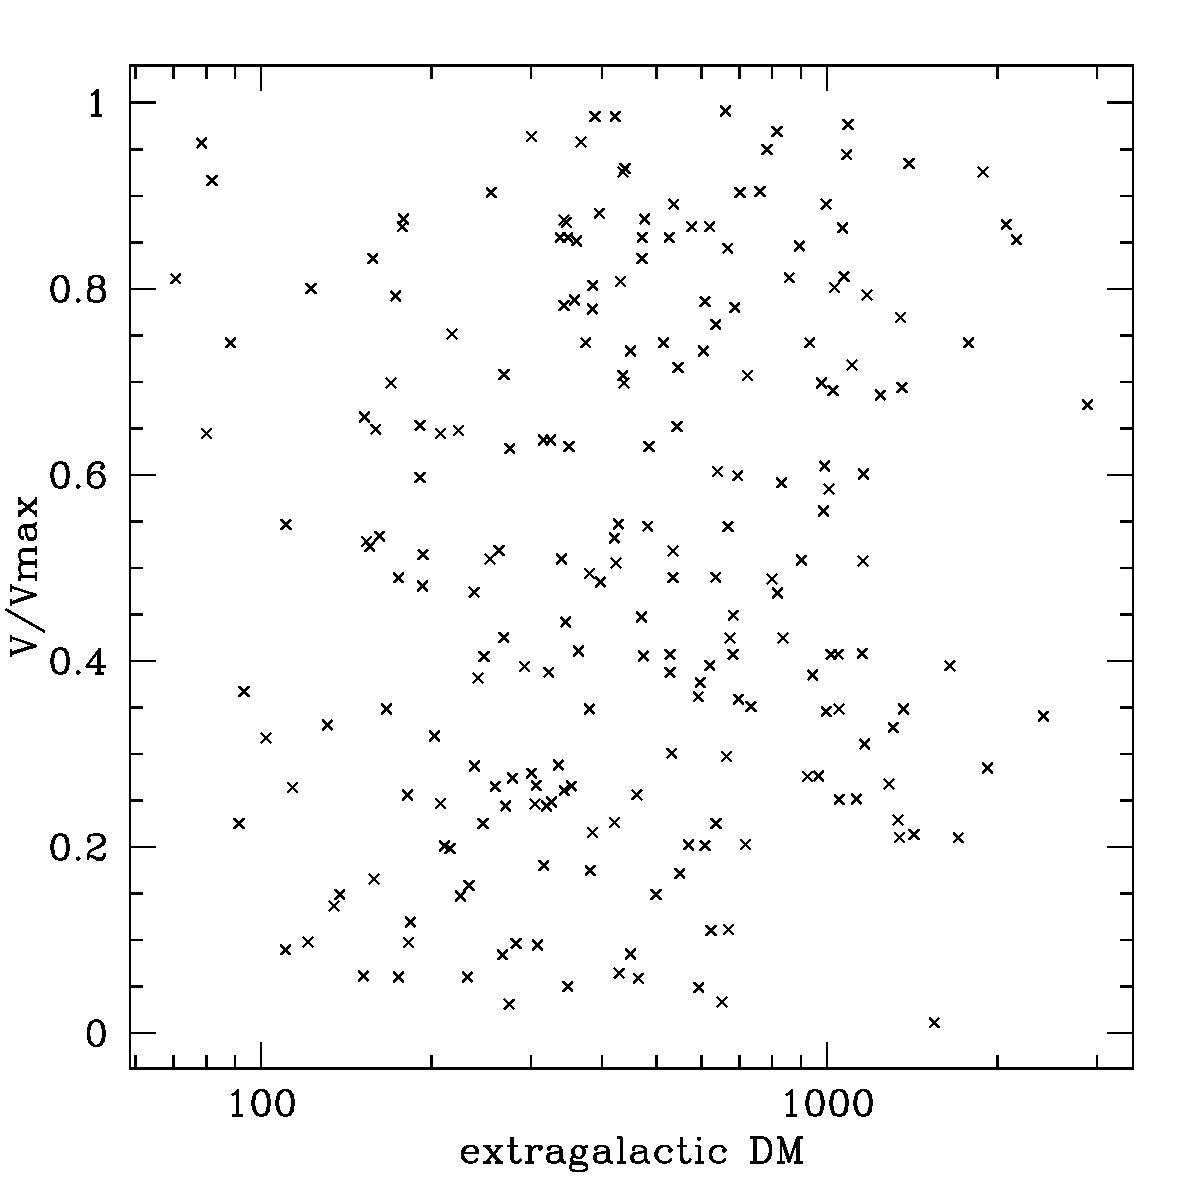
\includegraphics[width=3.3in]{Figures/frbdm.pdf}
}


  \frame{
    \frametitle{Vmax}
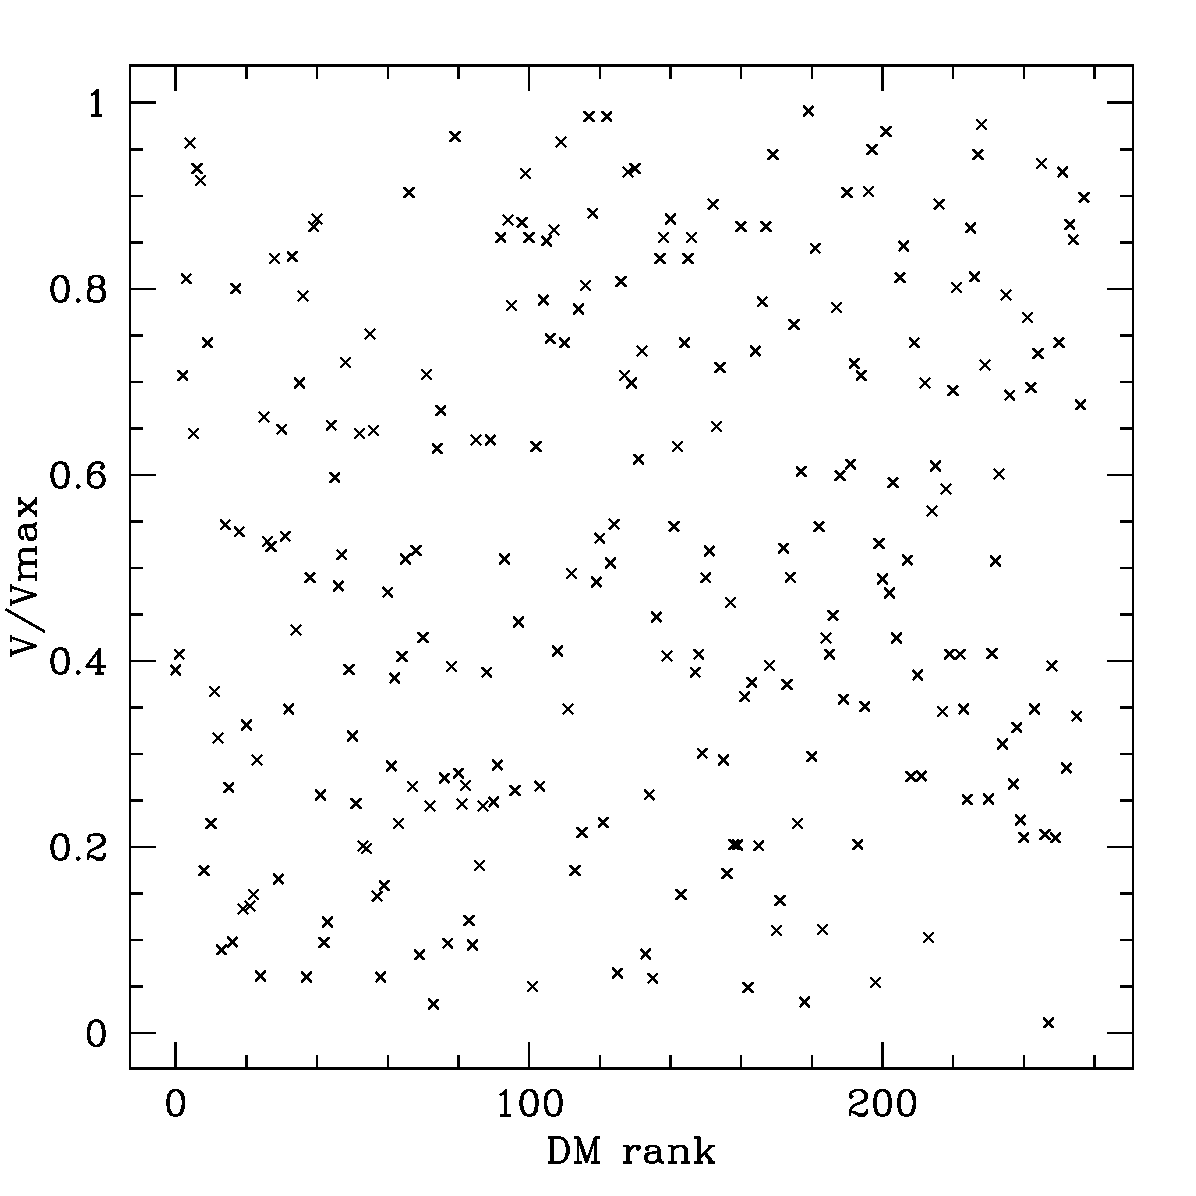
\includegraphics[width=3.3in]{Figures/frbdmrank.pdf}
}
  \frame{
\vspace{-0.5in}    \frametitle{DM}
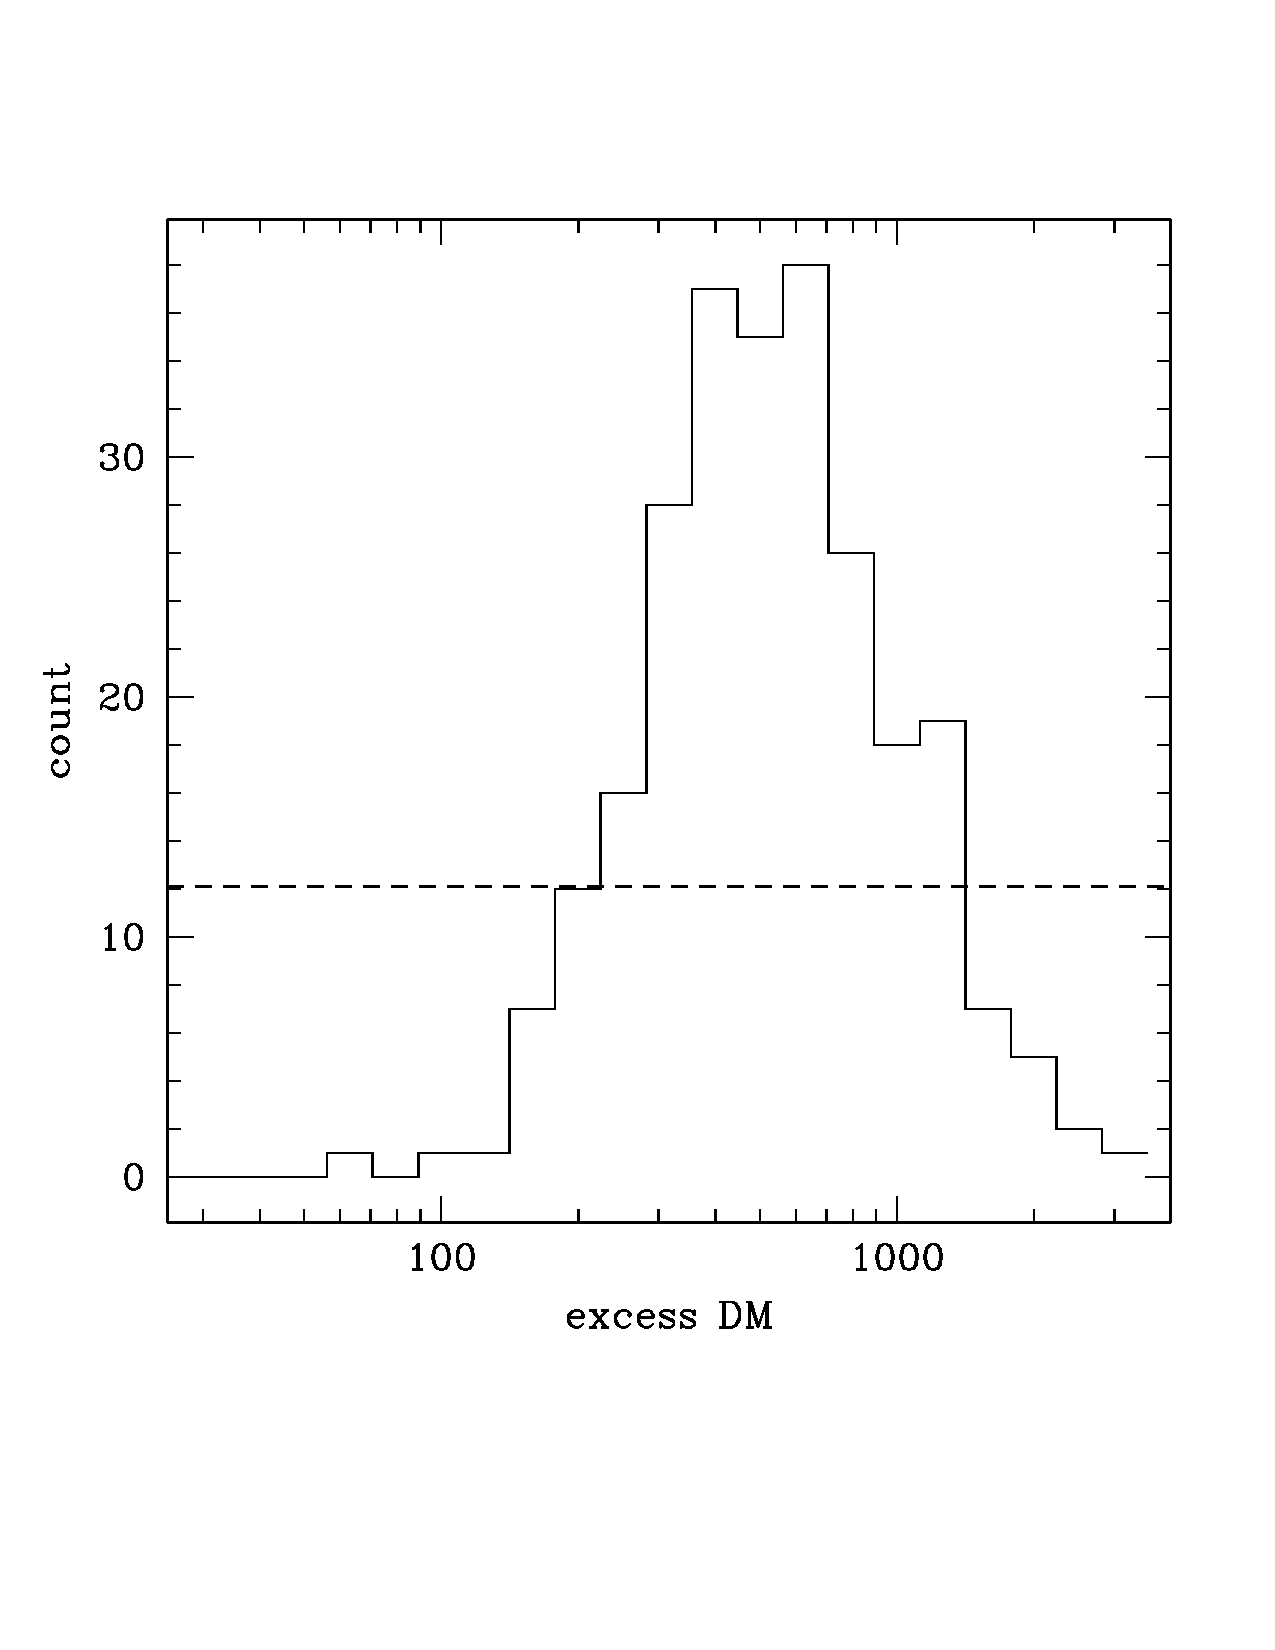
\includegraphics[width=3.6in]{Figures/frbdmhist.pdf}
}

  \frame{
\vspace{-0.5in}
    \frametitle{Luminosity function}
    \begin{itemize}
      \item for IGM, $z\sim $DM/1000
      \item low DM events measure faint end
      \item high DM events measure bright end
      \item cosmic evolution important around DM$>500$
      \item evolution small at DM$<400$
      \item $N(>L)=\sum_{>L} 1/V_{\rm max}$ (Eke+ 1996)
     \end{itemize}
  }


  \frame{
    \frametitle{Luminosity}
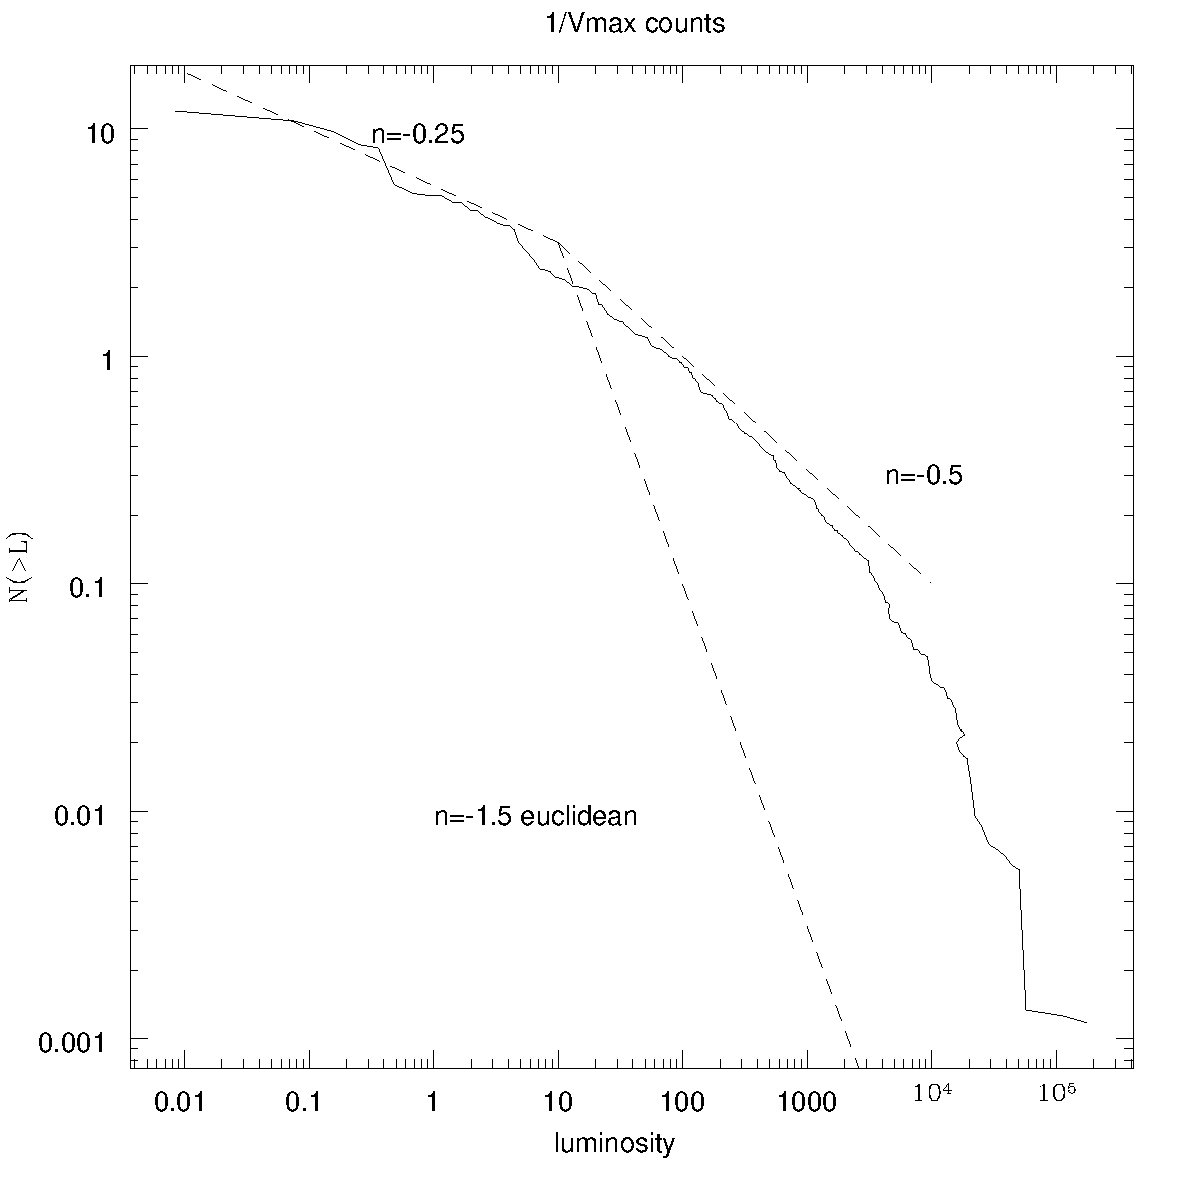
\includegraphics[width=3.4in]{Figures/lfn.pdf}
}


  \frame{
%\vspace{-0.5in}
    \frametitle{More bright bursts?}
    \begin{itemize}
      \item Luminosity function predicts V/Vmax distribution
      \item strong deviation from -3/2 implies more bright bursts than observed
     \end{itemize}
  }

  \frame{
 \vspace{-0.25in}
   \frametitle{V/Vmax}
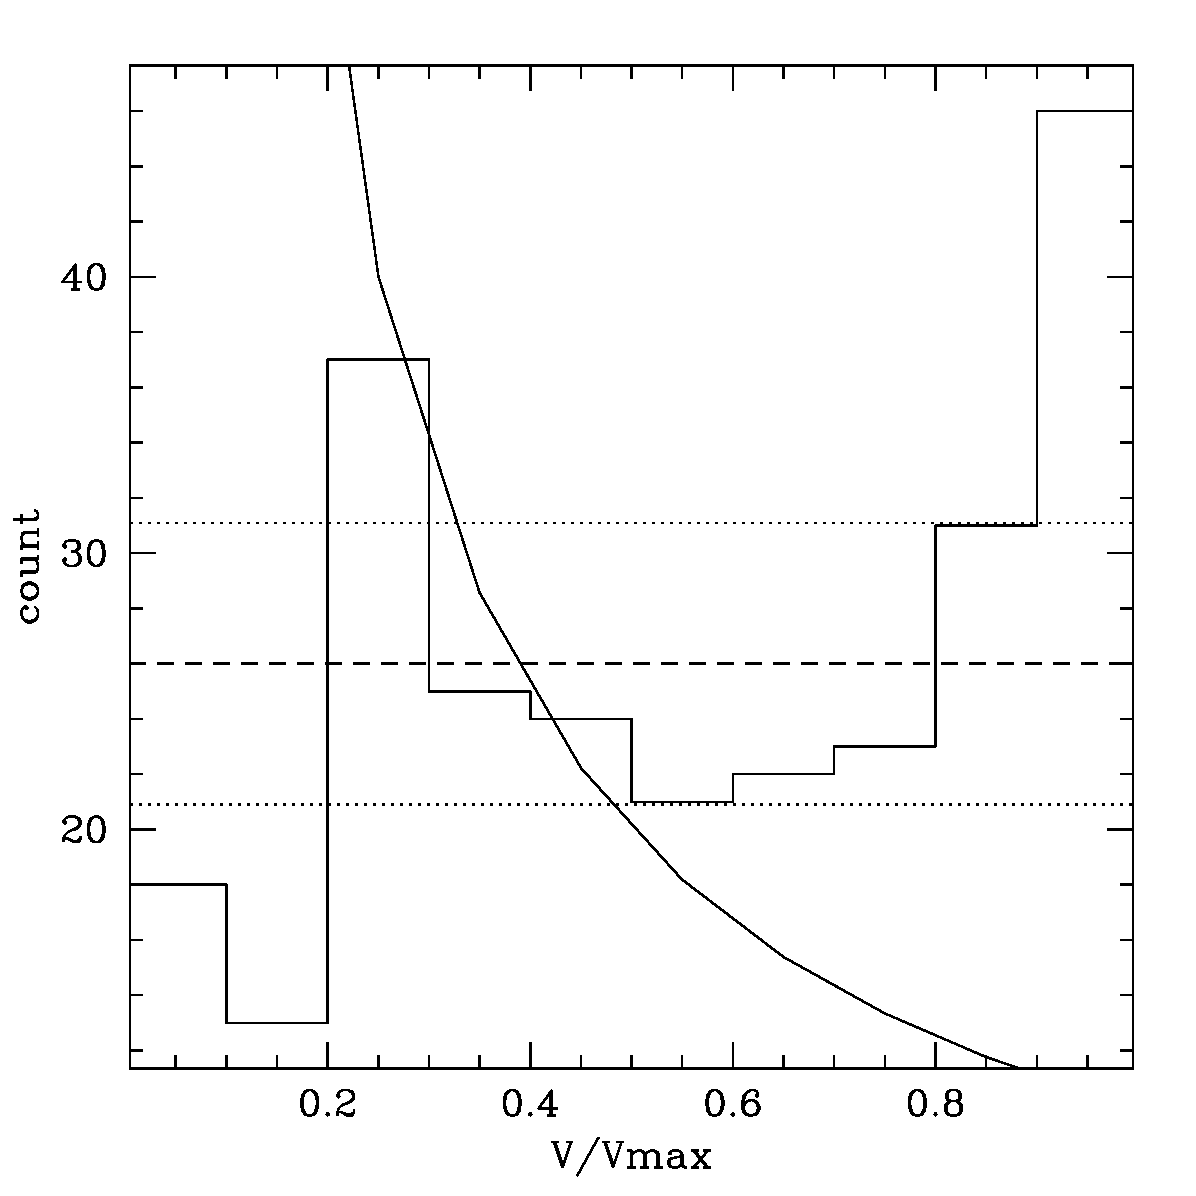
\includegraphics[width=3.4in]{Figures/frbvmax.pdf}
}

  \frame{
\vspace{-0.5in}
    \frametitle{YMW correction}
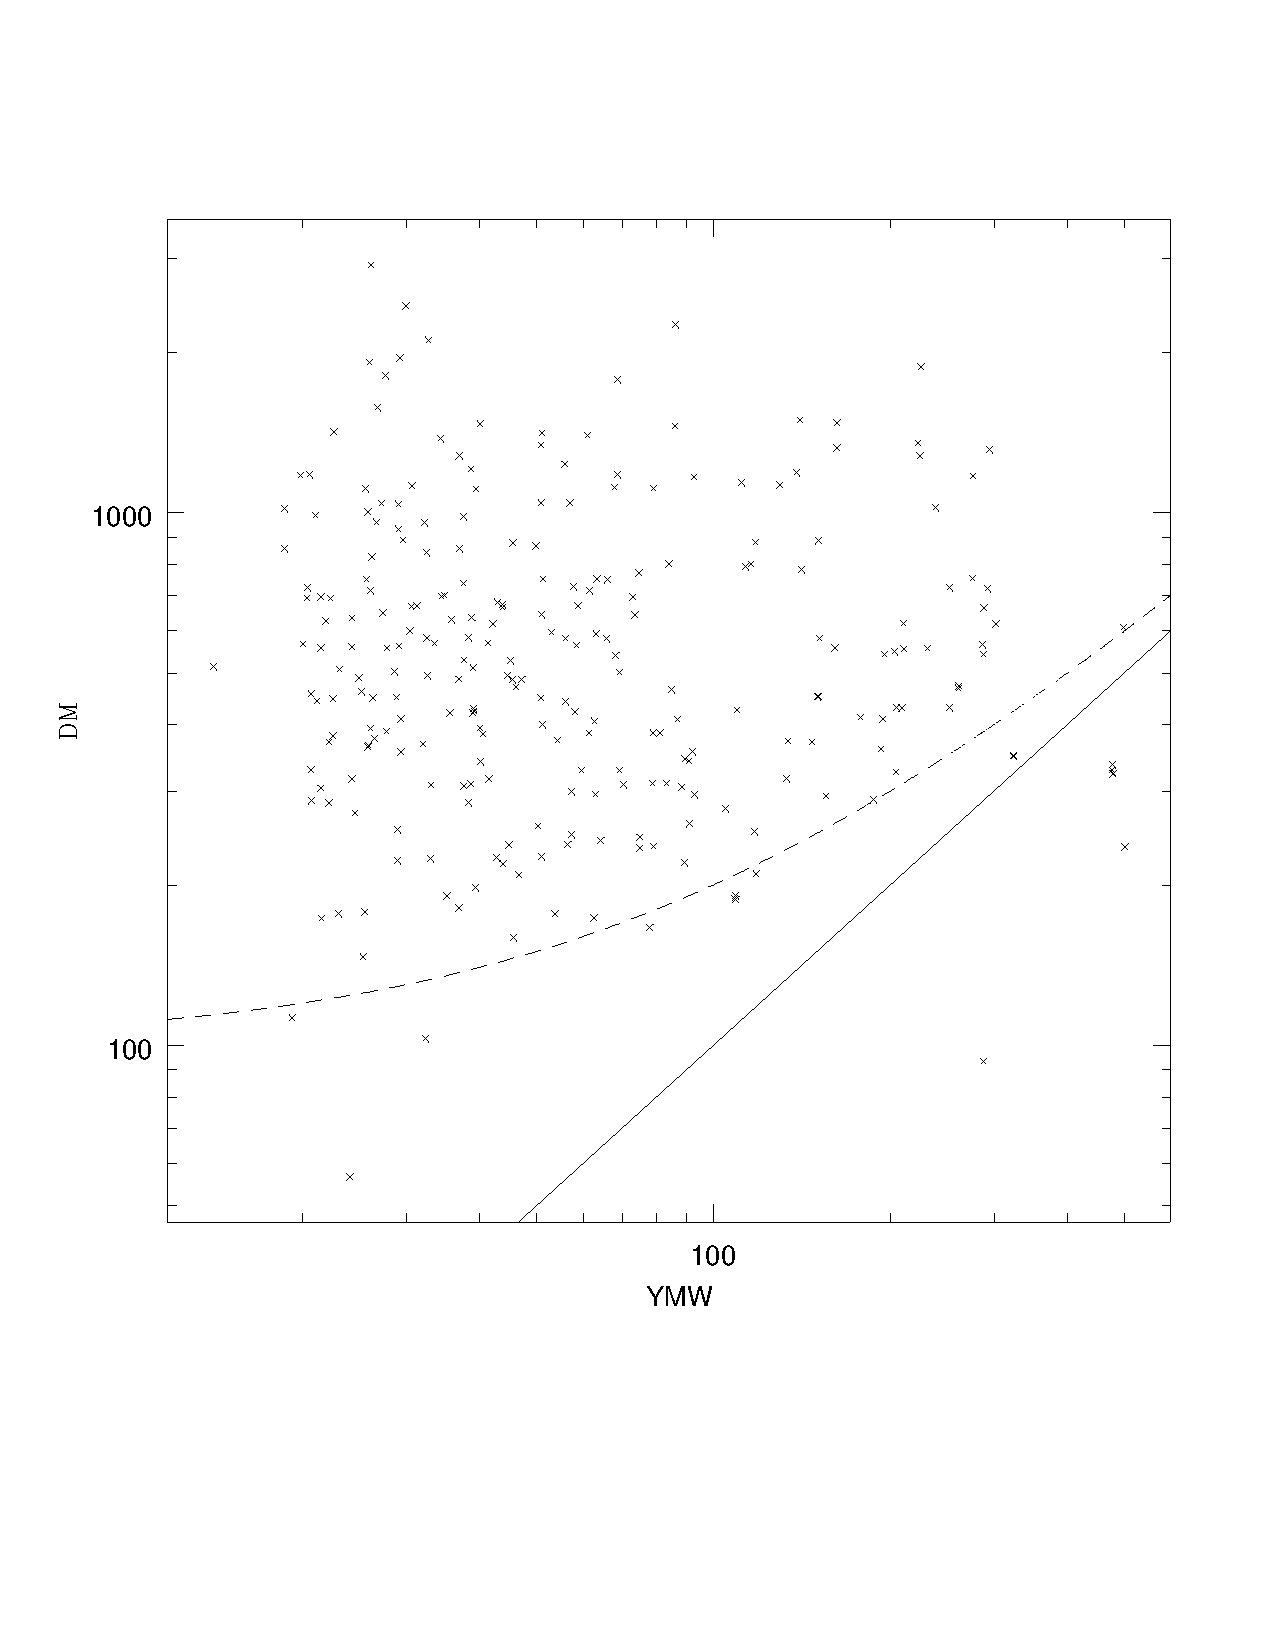
\includegraphics[width=3.4in]{Figures/dmymw.pdf}
}

\frame{
\vspace{-0.5in}
    \frametitle{Conclusions}
    \begin{itemize}
        \item IGM DM negligible allowed by data
        \item distance dominated by DM only allowed if Luminosity
          function is $L^{-1.5}$ AND CHIME sample is
          order of magnitude incomplete at low DM, AND galactic DM
          variation hidden by scattering.
        \item shallow luminosity function inferred from DM
          distribution not allowed by Vmax, also out-of-beam data
        \item plausible redshift $z\sim 0.05$(1902.10120), should yield strong cross
          correlation with 2MRS, SDSS main sample.
        \item in tension with unpublished ASKAP identifications
        \item need to better understand CHIME DM selection
        \item calibrate high SNR from baseband? 
     \end{itemize}
  }


\end{document}
